\chapter{Hauptteil}
\label{c:hauptteil}

This chapter will first outline the problems that constitutes the main portion of this work. Each problem is described separately starting with the available data sources followed by a detailed description of the proposed solutions. After that, the proposed solutions are evaluated by empirical means and the results are presented. Performance studies are conducted to provide suitable recommendations concerning the real world application.



\section{Erlaeuterung der Aufgabenstellungen}
\label{s:erlaeuterungaufgabe}




\section{Aufgabe 1: Implementierung einer Browser-Extension zur Anzeige von Datenschutzinformationen im PlayStore}
\label{s:implementierungextension}

\subsection{Anwendungsszenario}
\label{ss:anwendungsszenario}

QUELLE STATISTIK? 

Während vor einigen Jahren Applikationen hauptsächlich auf eigenen Webseiten zum Download angeboten wurden, haben sich die
AppStores mitlerweile durchgesetzt. Vorteile für diese Plattformen sind unter anderem: erleichterter Zugang, Vergleiche mit anderen Applikationen und individuelle Empfehlungen. Bei der Wahl für eine bestimmte Applikation achten Nutzer auf Aspekte, wie Preis, Anzahl der Downloads und Bewertungen von anderen Nutzern.

Immer wichtiger aber auch die Frage: Welche Daten gebe ich der Applikation frei und wie werden diese verarbeitet. Der PlayStore bietet zwar einen groben Überblick, welche Daten eine Applikation von dem Handy ausließt, aber nicht wie diese vom Anbieter verarbeitet werden.

Dadurch entstehen beim Nutzer Fragen, welche der Playstore nicht beantwortet:
 \begin{enumerate}
 	\item Handhabung der Daten: Wie werden die Daten verarbeitet und an wen werden diese weitergeleitet? Wird ein Profil anhand der Daten erstellt? Welche Sicherheit besteht bei der Übertragung der Daten?
 	\item Vor- und Nachteile der Datenverarbeitung: Kann der Anbieter die Applikation dadurch komfortabler gestalten? Wird Werbung in der Applikation personalisiert? Besteht Gefahr vor Missbrauch der Daten?
 	\item Kontrolle über die Daten: Welche Möglichkeiten stehen zu Verfügung im Falle von Nichteinverständnis? Ist der Umgang mit den Daten nach der Installation noch einschränkbar. Kann der Nutzer die Verwendung der Daten verbieten und trotzdem die App weiterhin nutzen?
 \end{enumerate}


\subsection{Anforderungsanalyse}
\label{ss:anforderungsanalyse}

\subsubsection{Funktionale Anforderungen}

Aus den Fragen die bei dem Anwendungsszenario entstanden sind werden funktionale Anforderungen gebildet um konkrete Aufgaben für die Extension zu schaffen. -Anforderungen in TEXTFORM-

-Direkt bei Apps in Anforderungen erwähnen
\begin{itemize}
	\item[/F10/] Erweiterung der Informationen im PlayStore:
	Der Nutzer hat die Möglichkeit im Browserfenster per Aktivierung bzw. Deaktivierung der Extension zusätzliche Datenschutzinformationen zu den angezeigten Applikationen ein- bzw. auszublenden.
	\item[/F20/] Anzahl von bedenklichen Eigenschaften einer Applikation:
	Zu jeder Applikation erhält der Nutzer ein Feedback von der Extension, wieviele Bedenken vorliegen.
	\item[/F30/] Darstellung von kritischen Eigenschaften einer Applikation:
	Eigenschaften einer Applikation, welche einen erheblichen Nachteil für den Nutzer darstellen oder einen möglichen Gesetzesverstoß beinhalten werden hervorgehoben.
	\item[/F40/] Abrufen von Details zu den Bedenken:
	Wird ein Bedenken angezeigt, kann der Nutzer direkt Erläuterung, Handlungsempfehlung sowie Vor- und Nachteile zu diesem Bedenken abrufen.
	\item[/F50/] Empfehlung bei Suchanfragen:
	Basierend auf den Bedenken einer Applikation kann der Nutzer die Suchanfrage so anpassen, dass ihm unbedenkliche Applikationen priorisiert angezeigt werden.
\end{itemize}

\subsubsection{Nichtfunktionale Anforderungen}

\begin{itemize}
	\item 
\end{itemize}

\subsection{Programmaufbau}
\label{ss:programmaufbau}

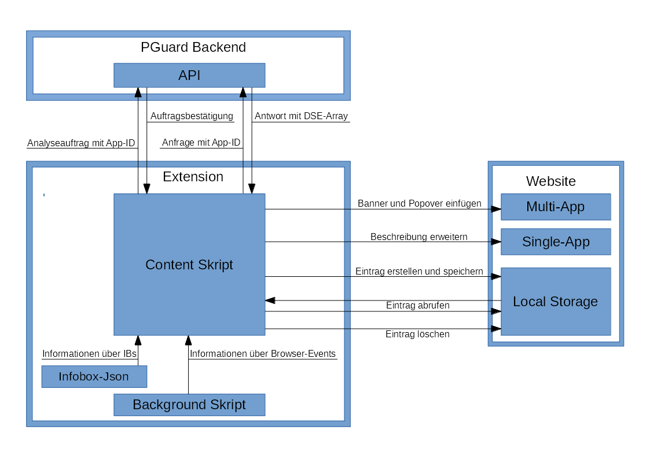
\includegraphics{pics/Aufbau.png}

\subsection{Ergebnis}
\label{ss:ergebnisseht1}


\subsection{Diskussion}
\label{ss:diskussionht1}










